\question{}
\begin{ابجد}
\item مسئله را به این شکل تعریف می‌کنیم:
\begin{itemize}
    \item \textbf{حالت‌ها}: می‌توانیم لیوان‌ها را در حالت کامل شماره‌گذاری کنیم (مثلا با شروع از ردیف پایین، و در هر ردیف از چپ به راست). در این صورت هر حالت، مجموعه لیوان‌هایی است که باقی مانده‌اند؛ بدیهی است که هر حالت زیرمجموعه حالت اولیه محسوب می‌شود.
    \item \textbf{کنش‌ها}: ضربه زدن به هر لیوانی در حالت فعلی که حداکثر یک لیوان به طور مستقیم روی آن قرار گرفته، و انداختن آن لیوان و تمام لیوان‌هایی که به طور مستقیم و غیرمستقیم بالای آن قرار گرفتند. (با توجه به محدودیت اعمال شده در انتخاب لیوان، نمی‌توانیم به لیوان‌هایی که دو لیوان روی آنها قرار گرفته ضربه بزنیم.)
    \item \textbf{هزینه کنش‌ها}: هزینه تمام کنش‌ها را مساوی و برابر با 1 در نظر می‌گیریم.
    \item \textbf{حالت(های) هدف}: هر مجموعه‌ای از لیوان‌ها که تعداد لیوان‌های ریخته شده در آن بیشتر از نصف کل لیوان‌های حالت اولیه باشد، حالت هدف محسوب می‌شود. (با این تعریف بعضی از حالت‌های هدف، ممکن نیستند؛ به عنوان مثال حالت $\{1, 2, 3, 4, 5, 7, 8, 9, 10\}$ را برای مسئله ترسیم شده در صورت سوال در نظر بگیرید. این حالت از دو نظر مشکل دارد: اول اینکه در حالت اولیه دو لیوان به طور مستقیم روی لیوان 6 قرار گرفته‌اند و نمی‌توانیم به آن ضربه بزنیم. همچنین اگر فرض کنیم به این لیوان ضربه زده باشیم، لیوان‌های 8، 9 و 10 گه به طور مستقیم و غیرمستقیم روی آن قرار دارند هم باید حذف می‌شدند. پس این حالت هدف قابل دستیابی نیست.)

\end{itemize}

\item اگر بخواهیم در هر مرحله تعداد لیوان‌هایی که ریخته می‌شوند را بیشینه کنیم، در حالت اولیه باید به راست‌ترین یا چپ‌ترین لیوان ردیف پایین ضربه بزنیم. هر مورد را جداگانه بررسی می‌کنیم:
\begin{itemize}
    \item \textbf{قابل قبول بودن}: با ارائه مثال نقض، نشان می‌دهیم که تابع $h$ قابل قبول نیست. \\
          فرض کنید در ابتدا یک هرم کامل با ارتفاع 14 داریم. این هرم در کل $\frac{14 \times 15}{2} = 105$ لیوان دارد. پس باید حداقل 53 لیوان بیفتند. حال فرض کنید تعدادی از لیوان‌ها را حذف کردیم و در نهایت به حالت زیر رسیدیم:
          \begin{figure}[H]
              \centering
              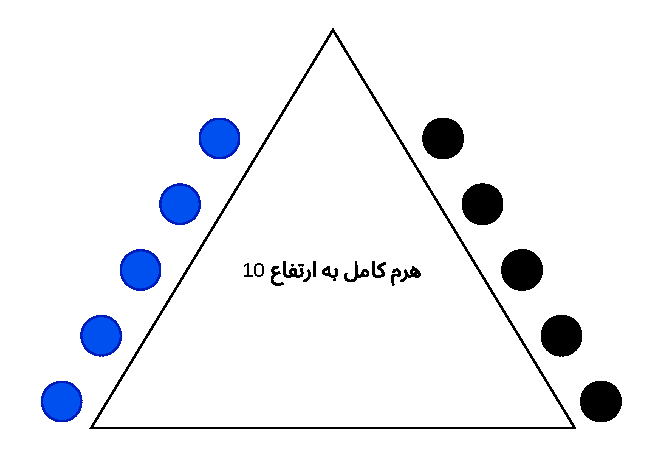
\includegraphics[width=0.5\textwidth]{assets/6_b_0.pdf}
          \end{figure}

          بهترین انتخاب در این حالت، انتخاب یکی از دو لیوان کناری در پایین‌ترین لایه هست، که در این صورت 5 لیوان فرومی‌ریزند. پس $\displaystyle \max_{c \in \text{targetable cups}(S)} f(c) = 5$.
          در این حالت $\frac{10 \times 11}{2} + 10 = 65$ لیوان داریم، پس $105 - 65 = 40$ لیوان تا الان افتاده‌اند و باید $53-40=13$ لیوان دیگر را بیندازیم. پس:
          \begin{equation*}
              h(S) = \frac{13}{5} = 2.6
          \end{equation*}
          حال فرض کنید یکی از دو لیوان مورد نظر را هدف قرار دهیم. سپس، می‌توانیم یکی از لیوان‌های کناری در لایه پایین هرم 10 تایی را هدف قرار دهیم. در این صورت 10 لیوان می‌افتند؛ در کل 55 لیوان تا الان افتاده‌اند و به حالت هدف رسیده‌ایم.
          \begin{equation*}
              h(S) = 2.6 \nleq h^*(S) = 2
          \end{equation*}
          پس تابع $h$ قابل قبول نیست.

    \item \textbf{یک‌نوا بودن}: با یک مثال نقض، نشان می‌دهیم که تابع مورد نظر یک‌نوا نیست. \\
          فرض کنید در ابتدا یک هرم کامل با ارتفاع 5 داریم:
          \begin{figure}[H]
              \centering
              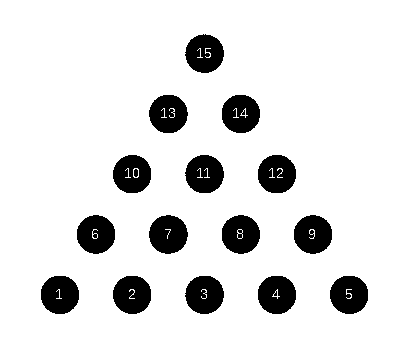
\includegraphics[width=0.5\textwidth]{assets/6_b_1.pdf}
          \end{figure}

          در هرم کامل، $\frac{5 \times 6}{2} = 15$ لیوان داریم و باید حداقل 8 لیوان فرو بریزند. فرض کنید 5 تا از لیوان‌های بالا حذف شده‌اند و به این حالت رسیدیم:
          \begin{figure}[H]
              \centering
              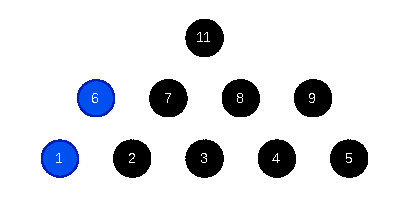
\includegraphics[width=0.5\textwidth]{assets/6_b_2.pdf}
          \end{figure}

          مقدار $\displaystyle \max_{c \in \text{targetable cups}(S)} f(c)$ در این حالت، به ازای لیوان شماره 1 (یا لیوان شماره 5) رخ می‌دهد که با ضربه زدن به آن، دو لیوان فرو می‌ریزند. (توجه کنید که در این حالت نمی‌توانیم لیوان‌های شماره 2 یا 4 را هدف قرار دهیم) بنابراین مقدار تابع $h$ در این حالت برابر است با:
          \begin{equation*}
              h(S) = \frac{3}{2}
          \end{equation*}
          به توپ شماره 1 ضربه زده (این اکشن هزینه 1 دارد) و به این حالت می‌رسیم:
          \begin{figure}[H]
              \centering
              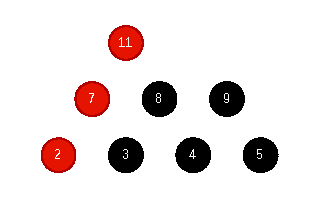
\includegraphics[width=0.5\textwidth]{assets/6_b_3.pdf}
          \end{figure}

          اکنون که یکی از لیوان‌های روی لیوان شماره 2 افتاده، می‌توانیم این لیوان را هدف قرار دهیم که در این صورت 3 لیوان می‌افتند. پس در این حالت:
          \begin{equation*}
              h(S') = \frac{1}{3}
          \end{equation*}

          داریم:
          \begin{equation*}
              h(S) - h(S') = \frac{3}{2} - \frac{1}{3} = \frac{7}{6} \nleq \mathrm{cost}(S \to S') = 1
          \end{equation*}
          بنابراین تابع $h$ یک‌نوا نیست.
\end{itemize}

\item تابع اکتشافی $h'$ را به این شکل تعریف می‌کنیم:
\begin{align*}
    h'(S) = \begin{cases}
                2   & \text{\lr{S} حالت اولیه باشد} \\
                0   & \text{\lr{S} حالت هدف باشد}   \\
                0.5 & \text{حالت‌های دیگر}
            \end{cases}
\end{align*}

برای اثبات قابل قبول بودن $h'$ باید نشان دهیم:
\begin{equation*}
    \forall S : 0 \leq h'(S) \leq h^*(S)
\end{equation*}
برای حالت‌هایی به جز حالت اولیه، بدیهی است که این رابطه صحیح می‌باشد. \\
اگر ارتفاع هرم $n$ باشد، در کل $\frac{n(n+1)}{2}$ لیوان داریم و باید حداقل $\lfloor \frac{n(n+1)}{4} + 1 \rfloor$ لیوان فرو بریزند. همچنین در هر حالت، حداکثر $n$ لیوان را می‌توانیم بیندازیم، که البته می‌دانیم این کار تنها در یک حرکت ممکن است. پس:
\begin{equation*}
    h^*(S_0) \geq \frac{\lfloor \frac{n(n+1)}{4} + 1 \rfloor}{n} > \frac{\frac{n(n+1)}{4}}{n} = \frac{n+1}{4}
\end{equation*}
که $S_0$ حالت اولیه است. با فرض اینکه ارتفاع هرم اولیه حداقل 15 باشد، داریم $h^*(S_0) \geq 4$ و در نتیجه $h'(S_0) < h^*(S_0)$. \\
پس تابع $h'$ قابل قبول است. \\

برای نشان دادن اینکه این تابع یک‌نوا نیست، کافی است مثالی را تصور کنیم که از حالت اولیه $S_0$ به حالت $S$ می‌رویم. ($S$ حالت هدف نیست)
\begin{equation*}
    h'(S_0) - h'(S) = 2 - 0.5 = 1.5 \nleq  \mathrm{cost}(S_0 \to S) = 1
\end{equation*}
پس تابع اکتشافی $h'$، یک‌نوا نیست.

\end{ابجد}